%% ggf:
% \part{Appendix}
% \label{part:appendix}

\chapter{Implementation Details}

\section{Determining the Lexical Scope}
\label{sec:app_lexical_scope}

\begin{figure}[!htp]
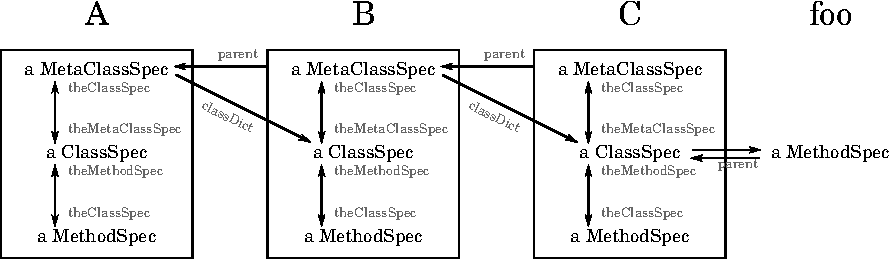
\includegraphics[width=\textwidth]{lexical_scope_app_ex.pdf}
\caption[Example: Detailed meta model]{Example: Detailed meta model.}
\end{figure}

\begin{figure}[!htp]
\begin{lstlisting}
MethodSpecification>>lexicalScopeIn: cls
    | enclosingClasses currentCls currentMetaClassSpec |
    enclosingClasses := OrderedCollection new.
    currentCls := cls.
    currentMetaClassSpec := self parent parent.

    enclosingClasses add: (currentCls := 
        (currentMetaClassSpec theClassSpec theMethodSpec 
            instantiations at: currentCls) first).

    [ currentMetaClassSpec parent isNil ] whileFalse: [
        currentMetaClassSpec := currentMetaClassSpec parent.
        enclosingClasses add: (currentCls := 
            (currentMetaClassSpec theClassSpec theMethodSpec 
                instantiations at: currentCls) first) ].

    ^ enclosingClasses
\end{lstlisting}
\caption[Determining the lexical scope of a method]{Determining all enclosing classes in the lexical scope of a method.}
\end{figure}

\section{Traits}
\label{sec:app_traits}

%%% Local Variables: 
%%% mode: latex
%%% End: 
